\tikzset{
    neuron/.style={
		circle,
		draw=black,
		minimum size=0.4cm,
		fill=blue,
	},	
    neuron dark/.style={
		circle,
		draw=black,
		minimum size=0.4cm,
		fill=TUMBlueDark,
	},	
	neuron missing/.style={
		draw=none, 
		fill=white,
		scale=1.0,
		text height=0.3cm,
		execute at begin node=\color{black}$\vdots$
	},
	label/.style = {draw=none, fill=none, rectangle, minimum height=1em, minimum width=1em},
	blockrx/.style = {draw, fill=white, rectangle, minimum height=1.5em, minimum width=6.25em},
	blocktx/.style = {draw, fill=white, rectangle, minimum height=1.5em, minimum width=13em},
	block/.style = {draw, fill=white, rectangle, minimum height=2em, minimum width=10em,rounded corners},
	blockthesis/.style = {draw, fill=gray!20, rectangle, minimum height=1.5em, minimum width=40em,rounded corners},
	block1/.style = {draw, fill=white, rectangle, minimum height=1.5em, minimum width=1.5em,rounded corners},
	tmp/.style  = {coordinate}, 
	sum/.style= {draw, fill=white, circle, node distance=1cm},
	mul/.style= {draw=none, fill=white, circle, node distance=1cm},
	input/.style = {coordinate},
	output/.style= {coordinate},
	pinstyle/.style = {pin edge={to-,thin,black}
	}
}

\begin{figure}[h]
    \centering
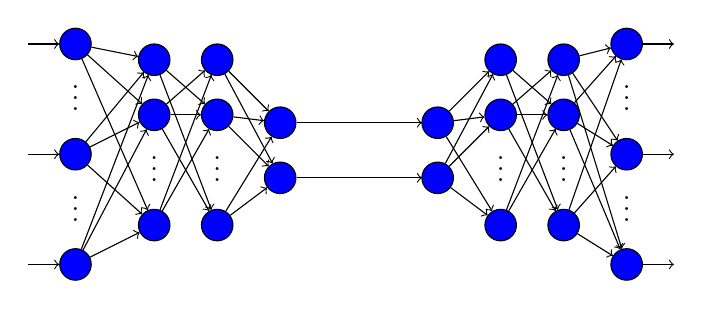
\begin{tikzpicture}
	%encoder
	\foreach \m [count=\y] in {1,missing,3,missing,5}
	\node [neuron/.try, neuron \m/.try] (input1-\m) at (0,2-\y*0.7) {};
	
	\foreach \m [count=\y] in {1,2,missing,4}
	\node [neuron/.try, neuron \m/.try ] (hidden1-\m) at (1,1.8-\y*0.7) {};
	
	\foreach \m [count=\y] in {1,2,missing,4}
	\node [neuron/.try, neuron \m/.try ] (hidden2-\m) at (1.8,1.8-\y*0.7) {};
	
	\foreach \m [count=\y] in {1,2}
	\node [neuron/.try, neuron \m/.try ] (output1-\m) at (2.6,1-\y*0.7) {};
	
	\foreach \i in {1,3}
	\draw [<-] (input1-\i) -- ++(-0.6,0);
	
	\foreach \l [count=\i] in {1,2}
	\draw [->] (output1-\i) -- ++(1.8,0);
%	node [above, midway] {$y_\i$};
	
	
	\draw [<-] (input1-5) -- ++(-0.6,0);

	%mesh1
	\foreach \i in {1,3,5} 
	\foreach \j in {1,2,4}
	\draw [->] (input1-\i) -- (hidden1-\j);
	
	\foreach \i in {1,2,4}
	\foreach \j in {2}
	\draw [->] (hidden1-\i) -- (hidden2-\j);
	
	\draw [->] (hidden1-2) -- (hidden2-1); 
	\draw [->] (hidden1-4) -- (hidden2-1); 
	
	\draw [->] (hidden1-1) -- (hidden2-4); 
	\draw [->] (hidden1-2) -- (hidden2-4); 
	
	\foreach \i in {1,2,4}
	\foreach \j in {1,2}
	\draw [->] (hidden2-\i) -- (output1-\j);
	
	%decoder
	\foreach \m [count=\y] in {1,2}
	\node [neuron/.try, neuron \m/.try ] (input2-\m) at (4.6,1-\y*0.7) {};
	
	\foreach \m [count=\y] in {1,2,missing,4}
	\node [neuron/.try, neuron \m/.try ] (hidden3-\m) at (5.4,1.8-\y*0.7) {};
	
	\foreach \m [count=\y] in {1,2,missing,4}
	\node [neuron/.try, neuron \m/.try ] (hidden4-\m) at (6.2,1.8-\y*0.7) {};
	
	\foreach \m [count=\y] in {1,missing,3,missing,5}
	\node [neuron/.try, neuron \m/.try] (output2-\m) at (7,2-\y*0.7) {};
	
	%outputs
	\foreach \i in {1,3,5}
	\draw [->] (output2-\i) -- ++(0.6,0);
	
	%mesh2
	\foreach \i in {1,2} 
	\foreach \j in {1,2,4}
	\draw [->] (input2-\i) -- (hidden3-\j);
	
	\foreach \i in {1,2,4}
	\foreach \j in {2}
	\draw [->] (hidden3-\i) -- (hidden4-\j);
	
	\draw [->] (hidden3-2) -- (hidden4-1); 
	\draw [->] (hidden3-4) -- (hidden4-1); 
	
	\draw [->] (hidden3-1) -- (hidden4-4); 
	\draw [->] (hidden3-2) -- (hidden4-4); 
	
	\foreach \i in {1,2,4}
	\foreach \j in {1,3,5}
	\draw [->] (hidden4-\i) -- (output2-\j);
	
	
	
	
\end{tikzpicture}    
\end{figure}